En el proceso de creación de la red 4G, se siguieron los siguientes pasos:

\begin{enumerate}
\item Descarga de la última versión de \textbf{Ubuntu}, \textbf{22.04 LTS}.
\item Grabación de la ISO en un pincho a través de \textbf{UNetbootin} y posterior instalación de Linux en el ordenador.
\item Instalación de los drivers de la \textit{Blade} siguiendo el manual de \textit{GitHub}:\\
 \url{https://github.com/Nuand/bladeRF/wiki/Getting-Started:-Linux}

\begin{lstlisting}
sudo add-apt-repository ppa:nuandllc/bladerf
sudo apt-get update
sudo apt-get install bladerf
\end{lstlisting}

\item Instalación de \textbf{srsran} siguiendo el manual de GitHub y las librerías \textbf{boost} y \textbf{libboost}:\\
\url{https://docs.srsran.com/projects/4g/en/latest/general/source/1_installation.html}\\
\url{https://docs.srsran.com/projects/4g/en/latest/getting_started.html}

\begin{lstlisting}
git clone https://github.com/srsRAN/srsRAN_4G.git
cd srsRAN_4G
mkdir build
cd build
cmake ../
make
make test
sudo make install
srsran_4g_install_configs.sh user
\end{lstlisting}

\item Modificación de los archivos de configuración que se encuentran en la ruta \textit{root/.config/srsran/}:
\begin{itemize}
	\item epc.conf
	\item enb.conf
	\item user_db.csv
\end{itemize}

En el archivo \textbf{enb.conf} se cambiaron los valores de \textbf{MCC} y \textbf{MNC} que están disponibles en las hojas de datos de las SIMs (y en la propia tarjeta SIM), y se establecieron sus valores correspondientes (\textbf{901-70}) para que correspondan con el IMSI. También se modificó el valor de la frecuencia central. cambiando el valor de \textbf{dl_earfcn}, para ello se utilizó \cite{earn}, estableciéndolo este valor 3050, lo que corresponde a un valor de frecuencia central \textit{downlink} de 2650.  Por último, se estableció el ancho de banda en 5MHz cambiando el valor de \textbf{n_prb} a \textbf{25}. Para mejorar el alcance de la red, se aumentó la ganancia de transmisor, cambiando el valor de \textbf{tx_gain} a 90.

En el archivo \textbf{epc.conf} se modificaron los valores de \textbf{MCC} y \textbf{MNC} (igual que en el caso anterior) y se añadieron los nombres de la red con:
\begin{lstlisting}
    full_net_name= NOMBRE
    short_net_name= NOMBRE
\end{lstlisting}

En el archivo \textbf{user_db.csv} se creó un usuario nuevo con la siguiente información:
\begin{lstlisting}
    nombre, mil (Auth), IMSI (aparece en las hojas de las sims),
    KEY (aparece en las hojas de las sims), opc,
    OPC(aparece en las hojas de las sims), 9000,
    sqn (poner todo a ceros, aunque cada vez que se levanta la red cambia automáticamente),
    7 (QCI), dynamic (IP_alloc)
\end{lstlisting}

\item Ahora que tenemos conectividad entre el enb y el epc, necesitamos que estos la tengan para el exterior, para eso ejecutamos el siguiente comando.

\begin{lstlisting}
    srepc_if_masq.sh enp0s25
\end{lstlisting}

\item Para levantar la red ejecutamos:
\begin{lstlisting}
    srsepc epc.conf
    srsenb enb.conf
\end{lstlisting}

\item Una vez obtenida la conexión a internet con la red 4G, nos bajamos los ficheros \textit{python} de control del coche para crear el servidor cloud e instalamos el servidor \textbf{MQTT Mosquitto} con los siguientes comandos:

\begin{lstlisting}
	sudo apt-get update
	sudo apt-get install mosquitto
\end{lstlisting}

\item Modificamos el fichero de configuración /etc/mosquitto/mosquitto.conf con las siguientes líneas:
\begin{lstlisting}
	persistence true
	persistence_location /var/lib/mosquitto/
	allow_anonymous true
	listener 1883 10.0.128.176
	bind_interface enp0s25
	log_type information
	log_type warning
	log_type error
\end{lstlisting}

\item Para comprobar el correcto funcionamiento del servidor \textbf{MQTT Mosquitto} nos  suscribimos a los tópicos básicos que se especifican en el manual de usuario del coche. Para ello, hacemos uso de la aplicación MyMQTT, si todo sale bien, se debería observar algo similar a la imagen \ref{mosquitto3}:

 \begin{figure}[H]
    \centering
    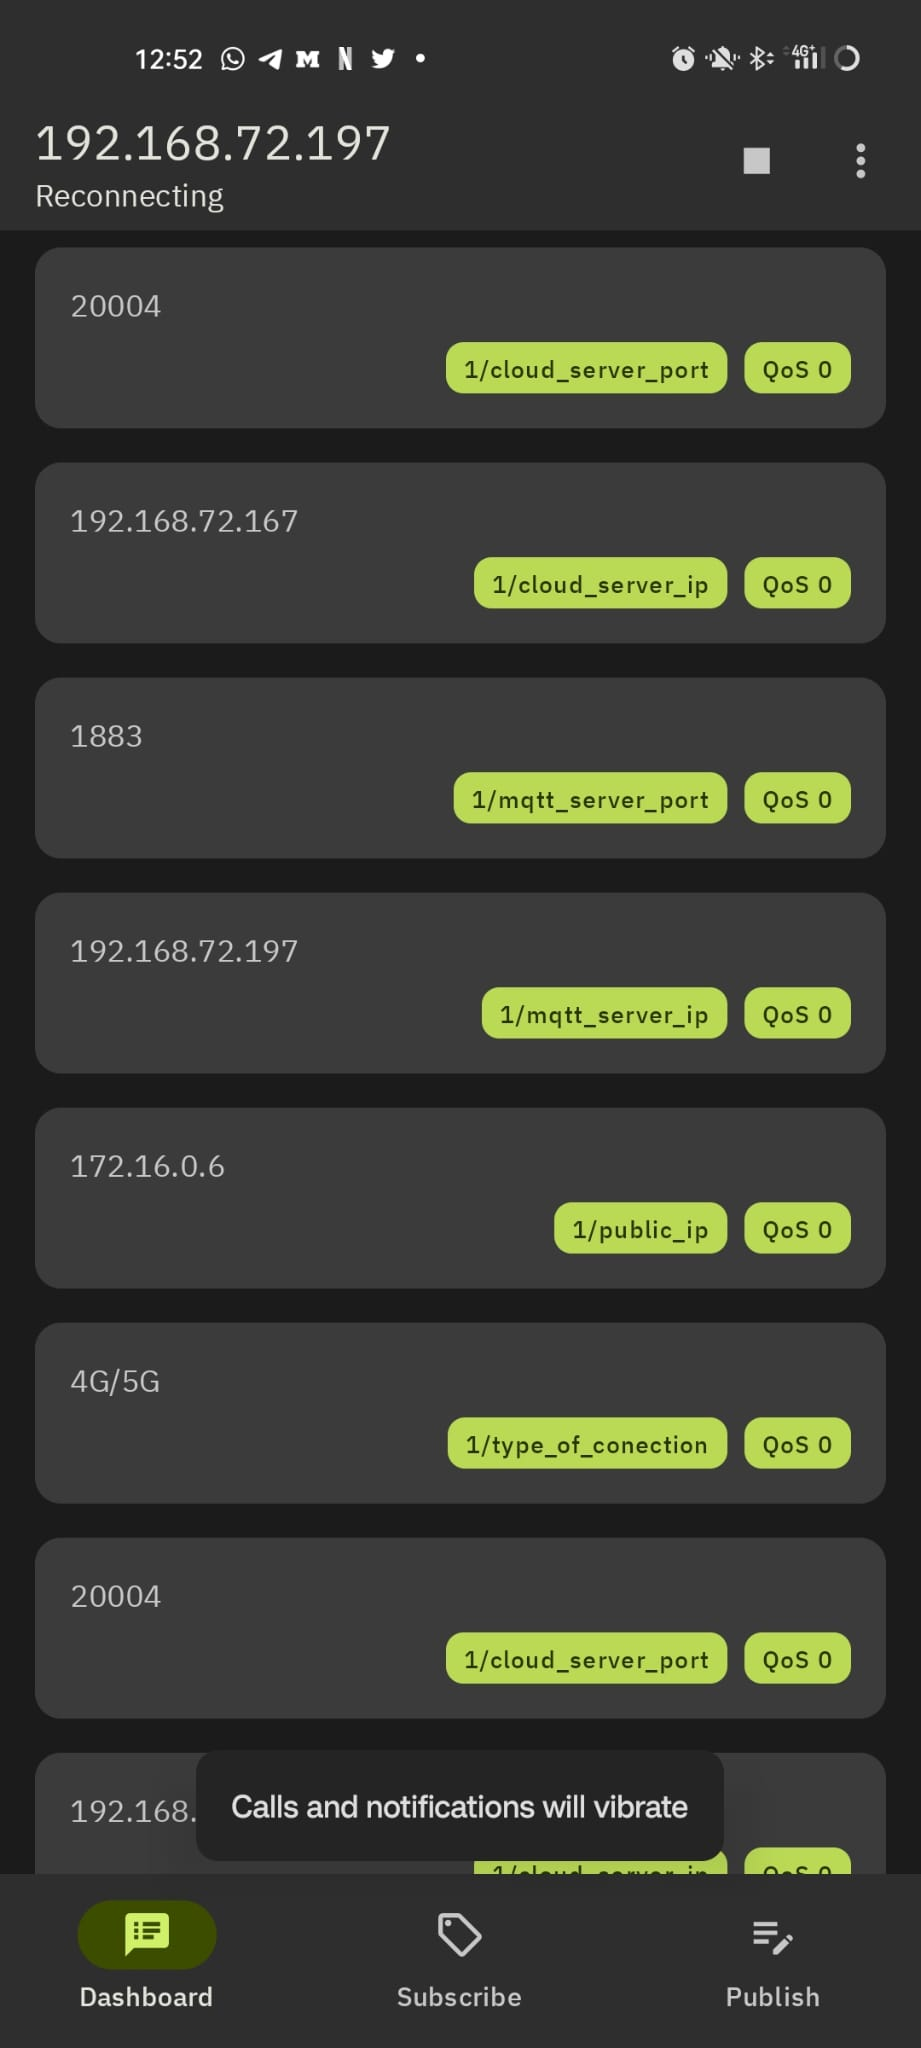
\includegraphics[width=0.53\textwidth]{Imagenes/Rendimiento/mosquitto3.jpeg}
    \caption{Información mostrada al iniciar la conexión}
    \label{mosquitto3}
\end{figure}

\item Por otra parte, en el dispositivo utilizado como cliente \textbf{MQTT Mosquitto} hay que suscribirse a los diferentes tópicos del vehículo, como podemos ver en la imagen \ref{mosquitto1}:

 \begin{figure}[H]
    \centering
    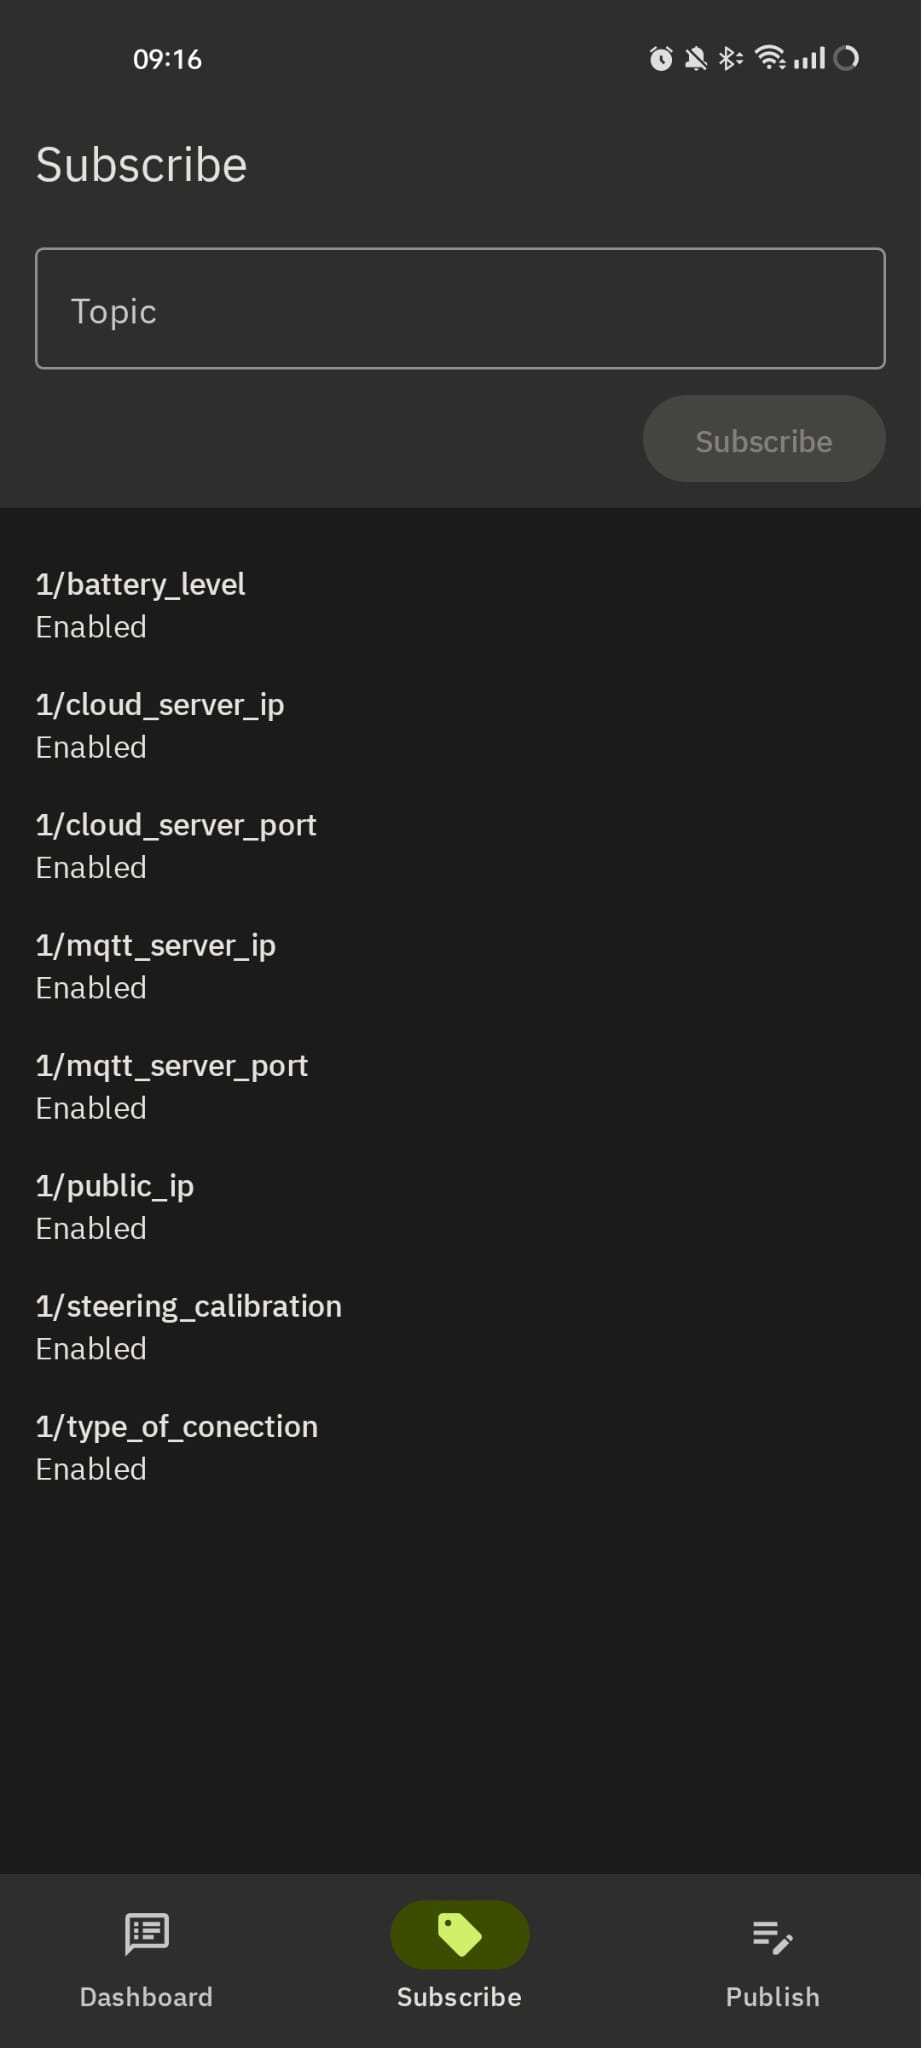
\includegraphics[width=0.53\textwidth]{Imagenes/Rendimiento/mosquitto1.jpeg}
    \caption{Suscripciones a los tópicos desde el móvil}
    \label{mosquitto1}
\end{figure}

Y, posteriormente, publicarlos como podemos ver en la imagen \ref{mosquitto2}

 \begin{figure}[H]
    \centering
    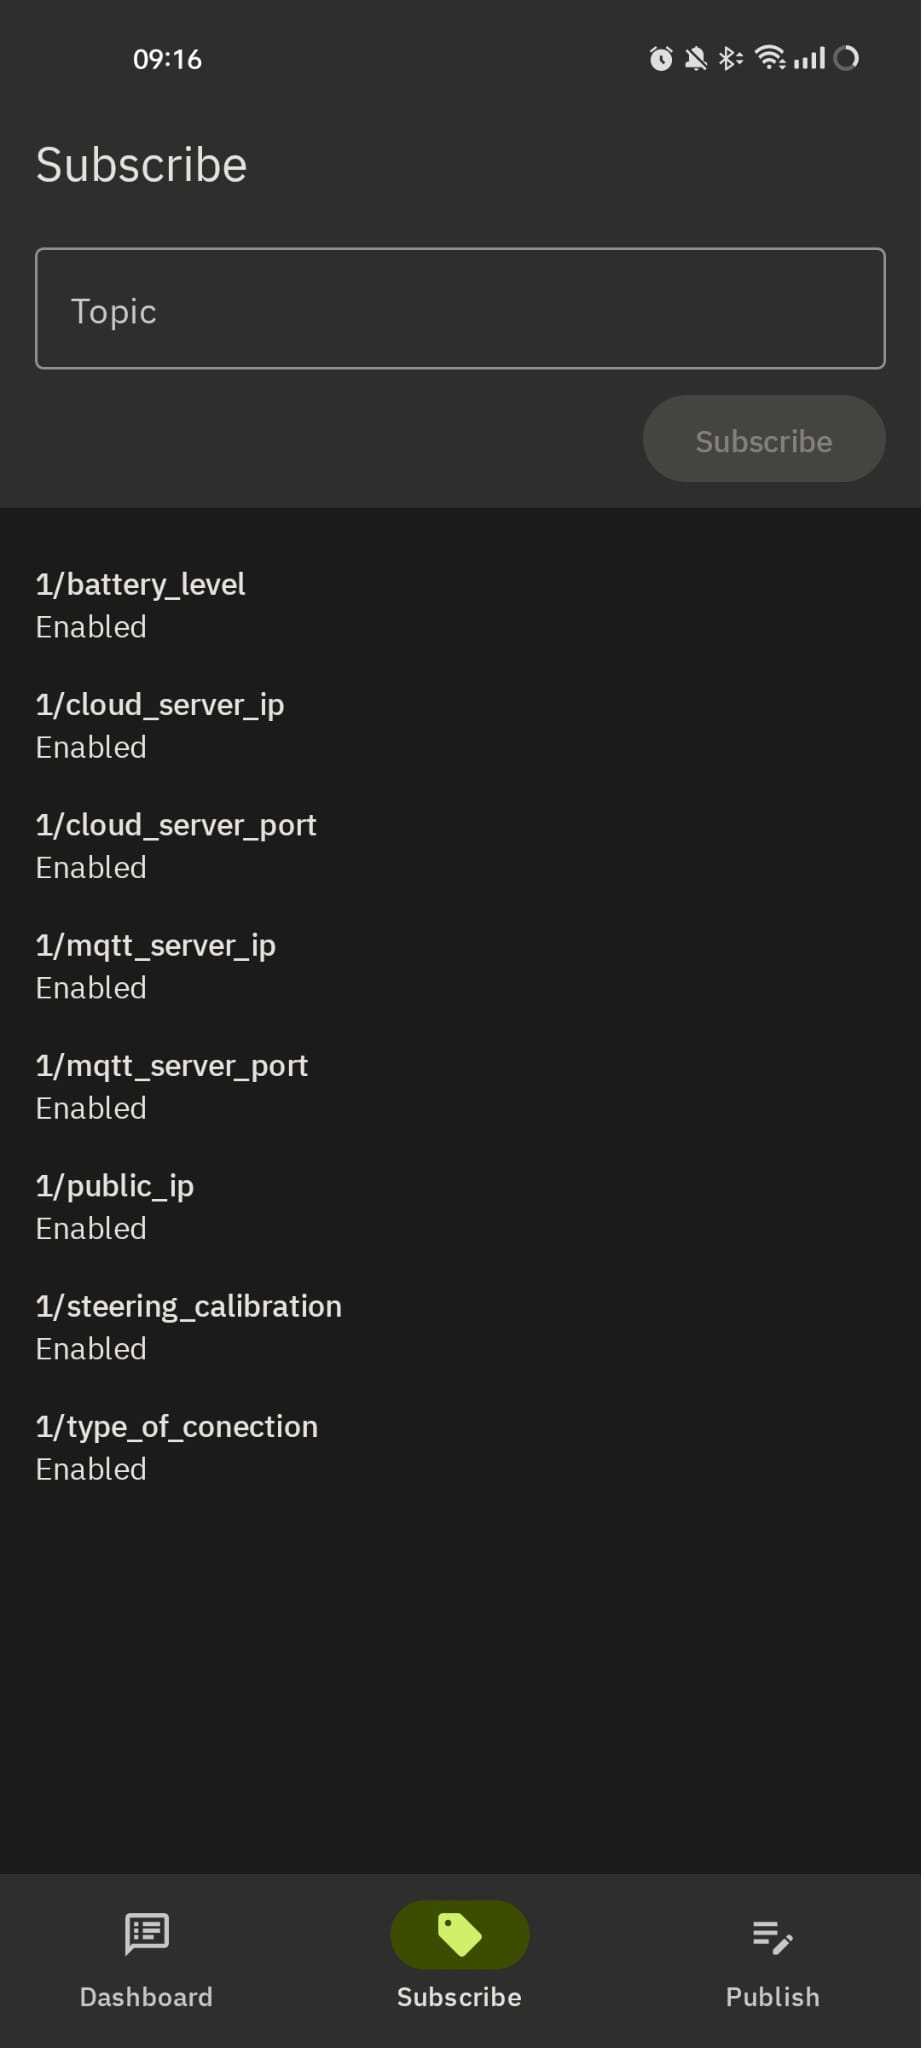
\includegraphics[width=0.53\textwidth]{Imagenes/Rendimiento/mosquitto1.jpeg}
    \caption{Publicación de comandos desde el móvil}
    \label{mosquitto2}
\end{figure}

\item Por último, para lanzar el servicio \textbf{MQTT Mosquitto} y otras acciones como relanzarlo, ver su estado o pararlo utilizamos los siguientes comandos:
\begin{lstlisting}
	sudo systemctl start mosquitto
	sudo systemctl status mosquitto
	sudo systemctl restart mosquitto
	sudo systemctl stop mosquitto
\end{lstlisting}

\end{enumerate}